\chapter{Dílčí části výukové sady}
Mnou vytvořená výuková sada se skládá ze tří vzájemně propojených částí:
\begin{itemize}[topsep=0pt]
    \setlength\itemsep{0em}
    \item Výukových videí,
    \item vytisknutelných materiálů,
    \item výukového portálu P3D.
\end{itemize}
Na jejich detailní popis se zaměřím v~této kapitole.

\section{Výuková videa}
Z~didaktického hlediska může být výukové video zpracované v souladu s doporučenými zásadami skvělým pomocníkem vyučujících, ale i studentů.
Před tvorbou samotného videa je nutné zvážit formát videa a připravit si scénář.
V~případě, že se rozhodnu pro video komentované, je nutné dbát i na kvalitu projevu.
Zároveň není žádoucí video příliš komplikovat a je zásádní dbát na stručné a jasné vysvětlení předváděného postupu či jevu.

S~tím se pojí časová náročnost přípravy, ale i samotného natáčení a zpracování videa.
Tvorba kvalitního výukového videa dokáže být velmi časově náročná a pokud člověk nemá s~videem dostatek zkušeností, může jeho výroba zahrnovat i několik nevydařených pokusů.

\subsection{Formát a struktura výukových videí}
Ještě před tím, než jsem začal vytvářet jednotlivá videa, jsem si musel odpovědět na několik důležitých otázek:
\begin{itemize}[topsep=0pt]
    \setlength\itemsep{0em}
    \item Jak budou videa koncipována? Bude se jednat o~krátká videa zaměřená na jeden konkrétní prvek, nebo budou delší a zaměřená na širší problematiku?
    \item Kam budu hotová videa umisťovat?
    \item Jak budou videa vypadat po grafické i technické stránce?
    \item Jaké bude jejich využití a účel?
\end{itemize}

Ve snaze najít odpověď na první z~nich jsem se zamyslel, jakým způsobem já sám vyhledávám informace.
Pokud potřebuji získat odpověď na konkrétní otázku v~dlouhém textu, mám možnost využít textového vyhledávání. 
U~videa ale žádná klávesová zkratka \It{Ctrl+F}\footnote{Zkratka běžně používaná pro vyhledávání v~dokumentech} zatím neexistuje -- musel bych tedy pomalu přeskakovat, až bych našel onu hledanou část.
Odpověď byla proto jasná -- krátká videa zaměřená na konkrétní prvek, jelikož díky nim budou studenti schopni najít řešení daného problému rychle a efektivně.

Úvaha nad druhou otázkou byla náročnější.
Na začátku jsem uvažoval nad umisťováním videí přímo na vlastní server, odkud by bylo možné je streamovat\footnote{Způsob přenosu dat, která jsou přenášena stabilním datovým proudem}.
V~takovém případě bych nebyl vázaný limitací žádné služby a pokud by mi nějaká funkcionalita chyběla, mohl bych si ji snadno vyrobit.
Následně jsem si však uvědomil, že tato varianta by konečnému divákovi nepřinesla žádný užitek, a proto jsem se rozhodl využít službu YouTube.
Její výhody pro koncového uživatele jsou stěžejní -- jedná se o~velkou platformu, která je mezi studenty i vyučujícími již velmi dobře známá.
Pro studenty by tedy nebyl žádný problém s~orientací, nebo dostupností obsahu (YouTube využívá vlastní CDN\footnote{Content delivery network, globální síť serverů určených pro distribuci obsahu}, díky které je zajištěná téměř stoprocentní dostupnost).

Posledním, avšak nesporně zásadním bodem bylo zvážení grafického designu a technických parametrů.
Design sám o~sobě prošel postupem času jistou proměnou, nicméně jsem se již od začátku snažil o~to, aby videa vypadala moderně a čistě, což studentům výrazně napomáhá v~orientaci v~nich.
Po technické stránce jsem se rozhodl držet rozlišení 1920x1080 při 60 snímcích za vteřinu a hlasitosti zvukové stopy normalizované na -14 LUFS, což je standardní hlasitost pro videa nahrávaná na YouTube.
Těchto parametrů se od vydání prvního videa držím, aby byla všechna co možná nejjednotnější.

Mimo to bylo nutné připravit strukturu videí.
Vzhledem k~tomu, že mají velmi stručně a srozumitelně představit optimální řešení daného problému, rozhodl jsem se v~otázce struktury držet třech zásadních bodů:
\begin{itemize}[topsep=0pt]
    \setlength\itemsep{0em}
    \item Úvod videa, kde je problematika každého z~nich stručně vysvětlena,
    \item hodnoty a parametry potřebné pro splnění úlohy,
    \item samotný postup tvorby daného prvku.
\end{itemize}

V~úvodu je krátce popsáno zaměření videa a smysl daného prvku, popř. postupu.
U~videí zaměřených na modelování následuje výčet potřebných hodnot a parametrů, které jsou pro vytvoření prvku, nebo součásti nezbytné.
Nakonec následuje názorná komentovaná ukázka samotného postupu.

\subsection{Podkresová hudba}
Podkresová hudba hrajeu výukových videí zásadní roli zejména v otázce udržení pozornosti studenta.
V~samotných začátcích jsem čerpal skladby z~platformy ncs.io, která poskytuje skladby k~volnému užití za předpokladu uvedení autora a zdroje.
Postupně jsem však dospěl k~závěru, že skladby použité u~některých původních videí jsou vzhledem k~výukové povaze obsahu nevhodné a rozhodl se styl volené hudby změnit. 
Změnil jsem i zdroj hudby a začal čerpat z~placené služby Artlist.io\cite{ARTLIST} umožňující licencování obrovského množství hudby mnoha různých žánrů a výběr v souladu s charakterem videa.

Při volbě skladby do podkresu se snažím volit žánry, které nebudou působit rušivě, příliš vážně, nebo naopak infantilně.
Hlasitost je vždy regulována tak, aby byl komentář ve videu dobře srozumitelný a hudba do něj nezasahovala.

\subsection{Náhledové obrázky}
V~případě videí P3D mají náhledové obrázky smysl zejména z~hlediska orientace.
Snažil jsem se proto, aby měly všechny jednotné rozložení i design a lišily se pouze obsahem a barvami, nikoliv strukturou.
\begin{figure}[htbp]
    \centering
    \begin{minipage}[b]{0.45\textwidth}
        \centering
        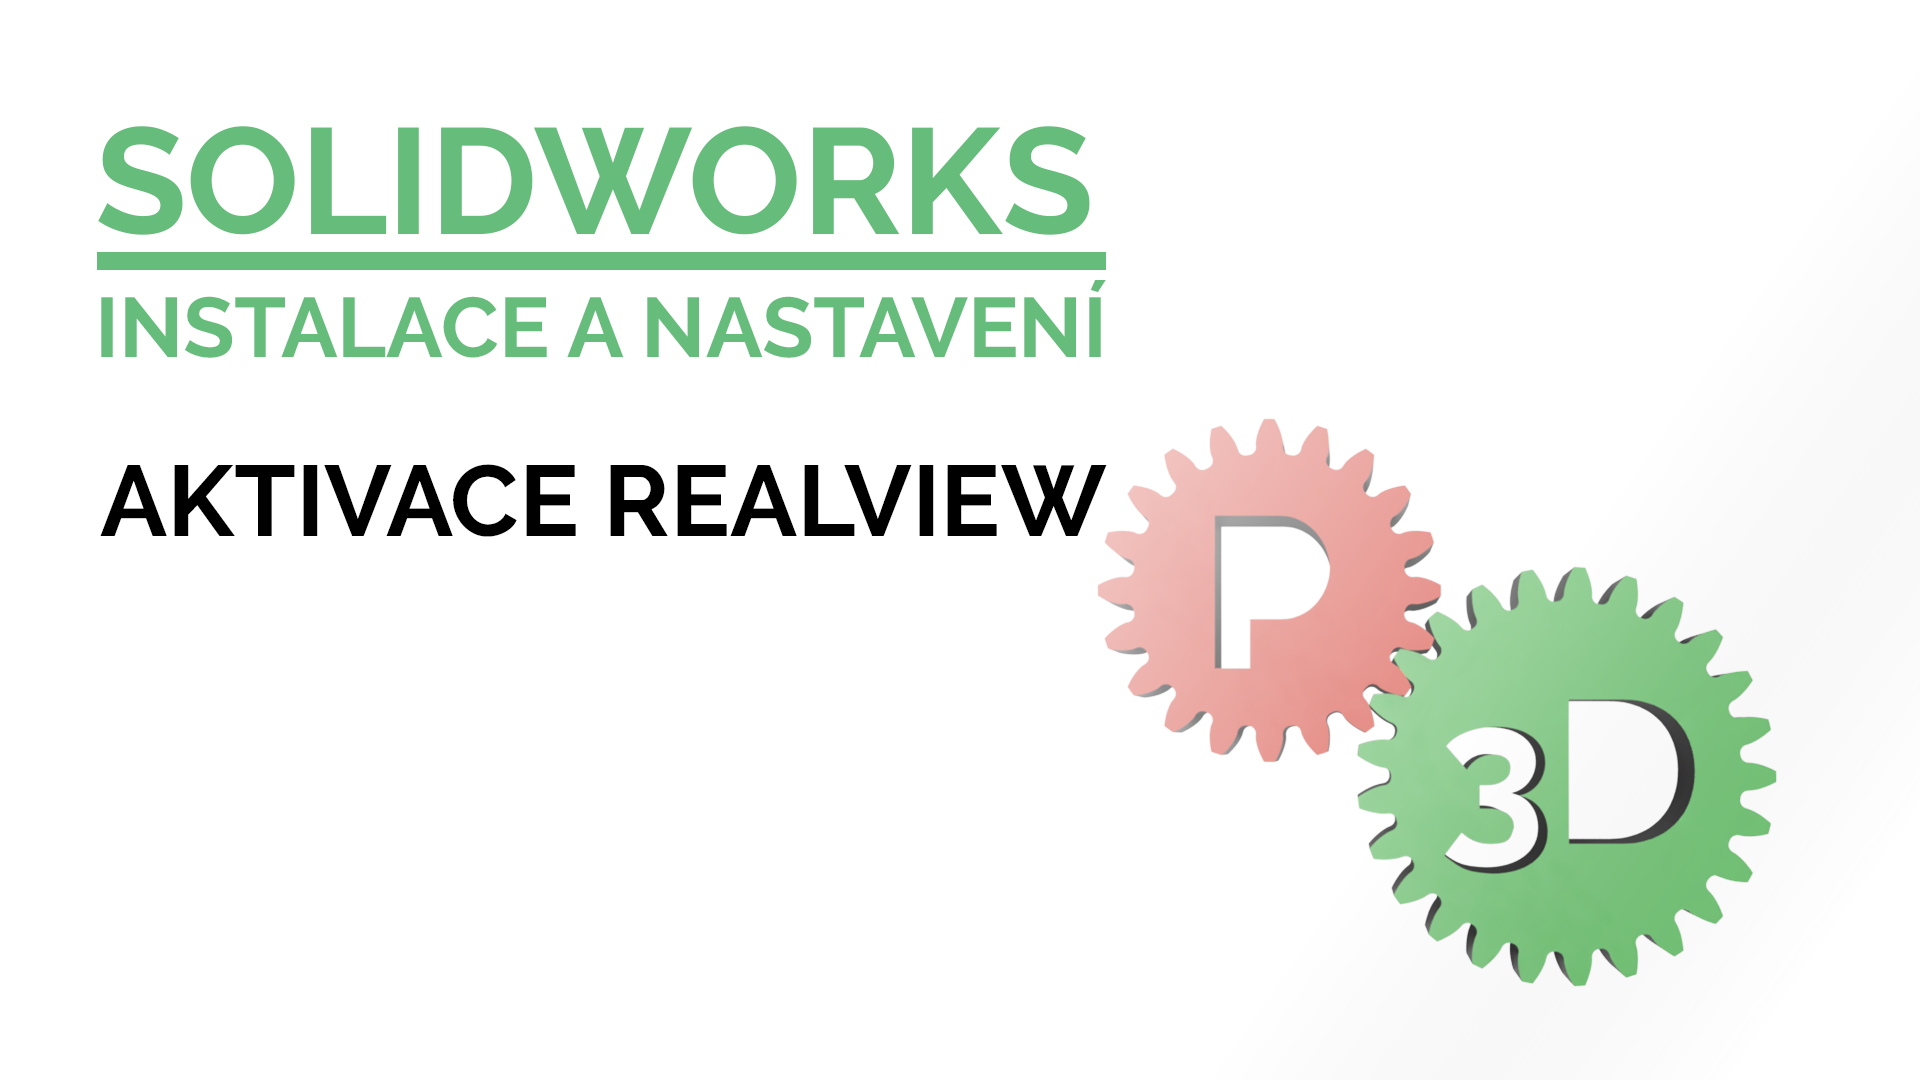
\includegraphics[width=0.8\textwidth]{img/020/aktivace-realview-thumbnail.png}
        \caption{Instalace a nastavení}
        \label{fig:thumb1}
    \end{minipage}
    \qquad
    \begin{minipage}[b]{0.45\textwidth}
        \centering
        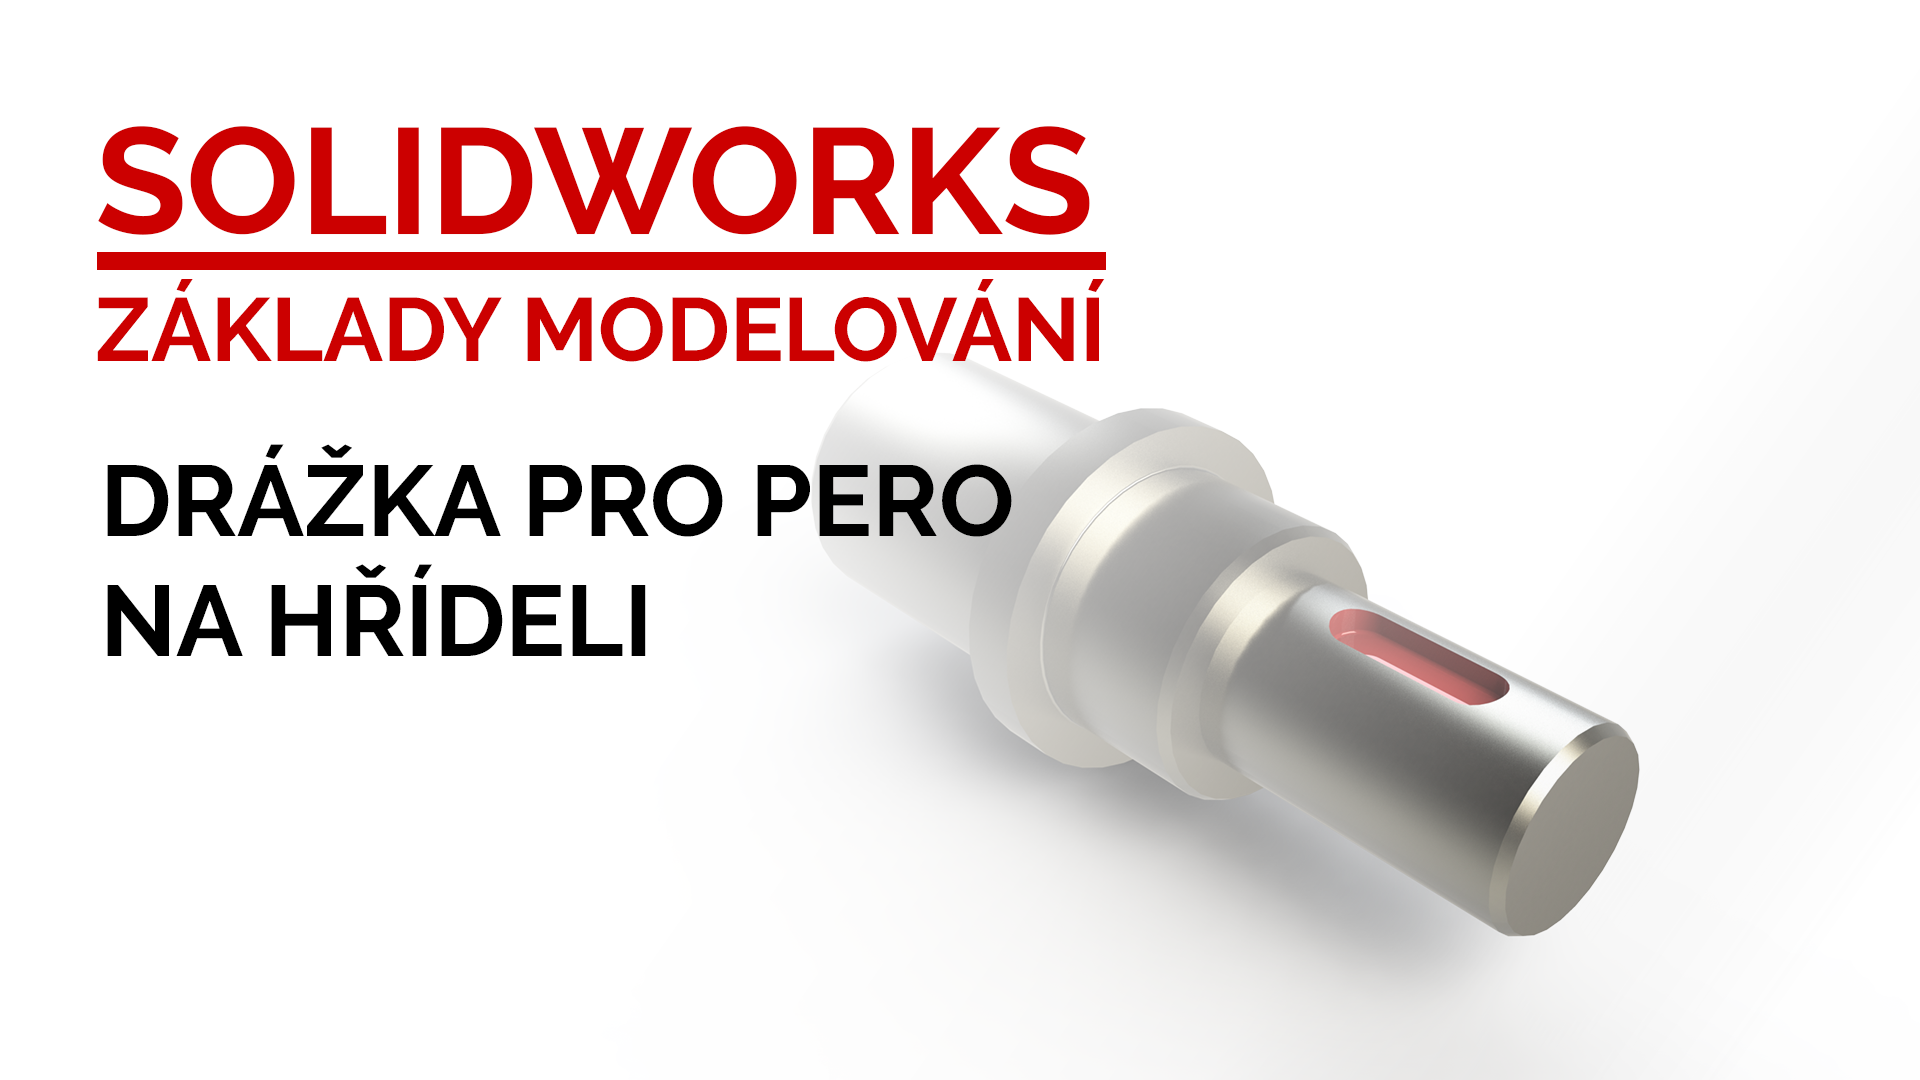
\includegraphics[width=0.8\textwidth]{img/020/perodr-hr-thumbnail.png}
        \caption{Modelování}
        \label{fig:thumb2}
    \end{minipage}
\end{figure}

\begin{figure}[htbp]
    \centering
    \begin{minipage}[b]{0.45\textwidth}
        \centering
        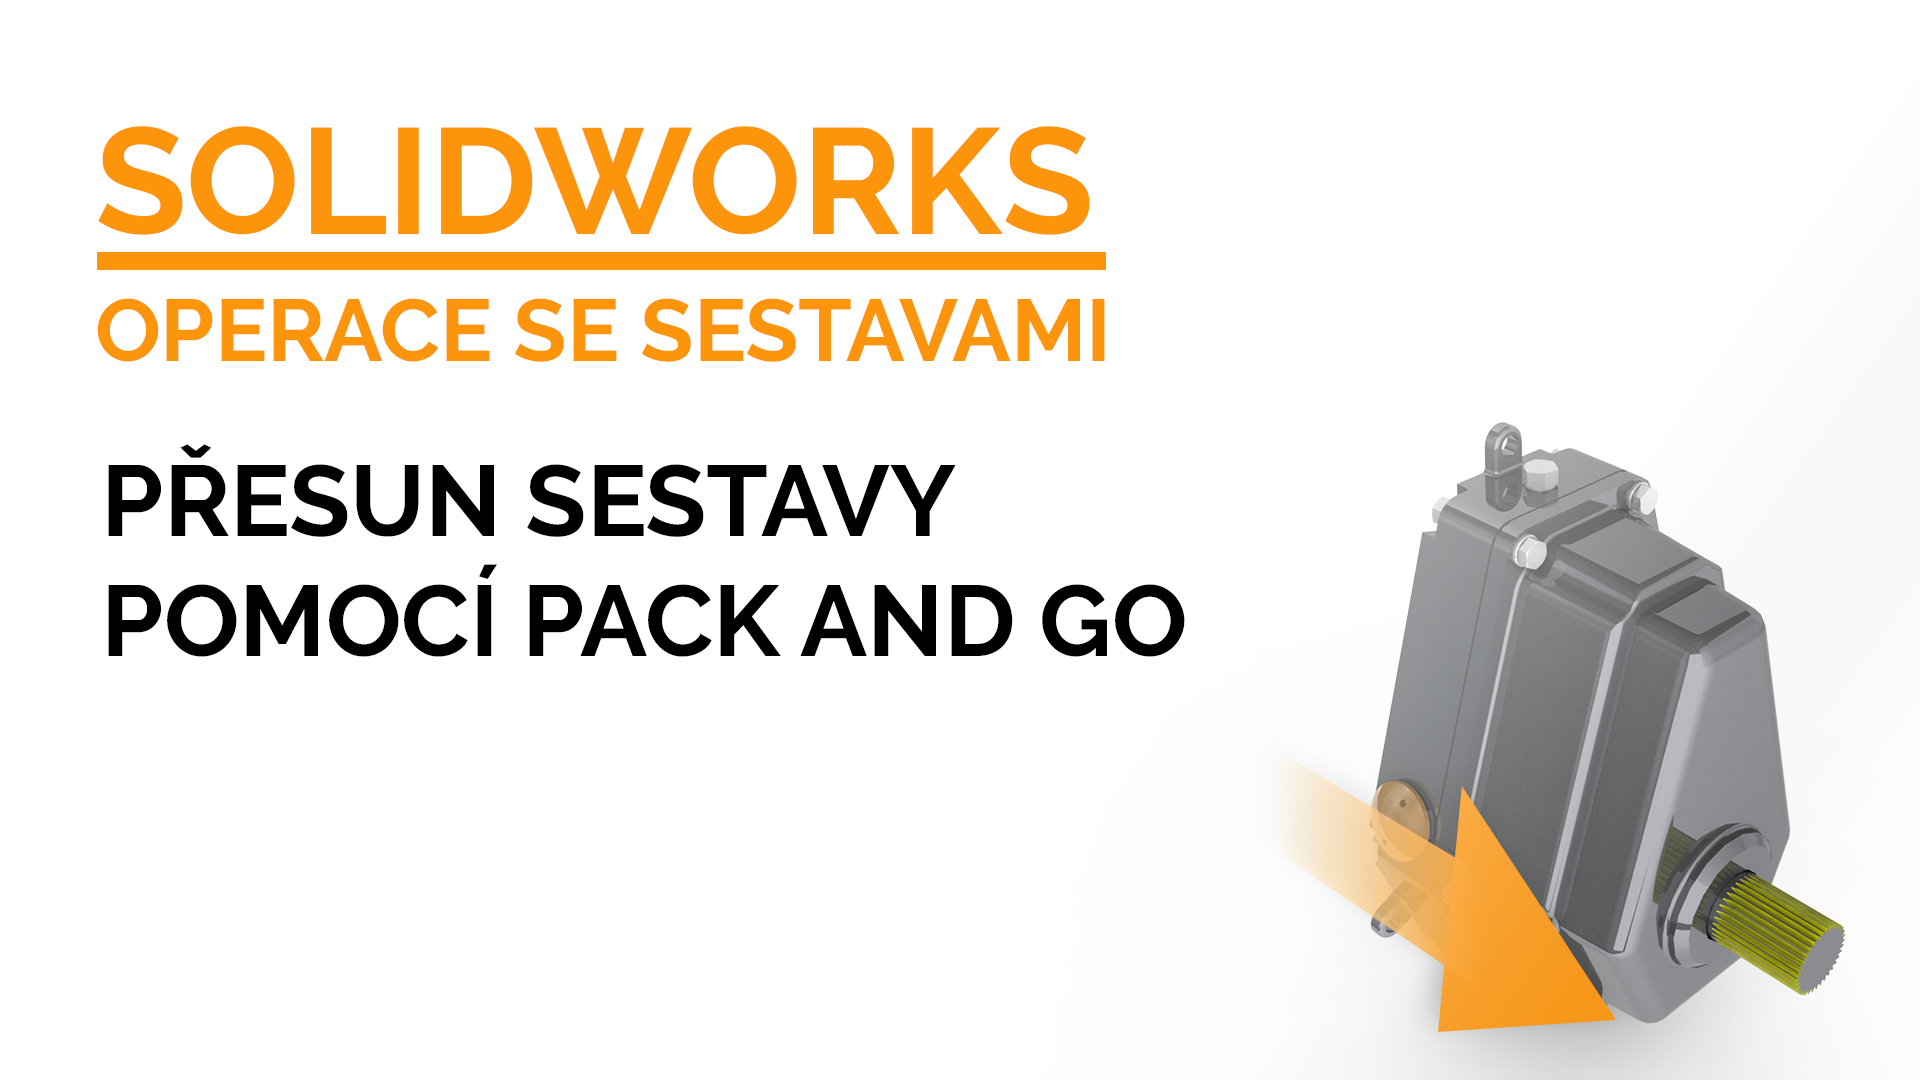
\includegraphics[width=0.8\textwidth]{img/020/pack-and-go-thumbnail.png}
        \caption{Sestavy}
        \label{fig:thumb3}
    \end{minipage}
    \qquad
    \begin{minipage}[b]{0.45\textwidth}
        \centering
        
\includegraphics[width=0.8\textwidth]{img/020/dwg-perodr-hr-thumbnail.png}
        \caption{Výkresová dokumentace}
        \label{fig:thumb4}
    \end{minipage}
\end{figure}

Jak můžete vidět na jednotlivých náhledech \ref{fig:thumb1}, \ref{fig:thumb2}, \ref{fig:thumb3} a \ref{fig:thumb4}, každý z~nich má v~levém horním rohu umístěný nadpis s~názvem série (resp. zaměřením), pod kterým se nachází konkrétní téma daného videa.
Pravá polovina náhledu je v~pozadí doplněná o~obrázek ilustrující dané téma (například hřídel s~drážkou pro pero).

Díky tomuto systému je studentovi již ve chvíli, kdy vidí náhled videa, jasné jeho téma, což podstatně usnadňuje orientaci.
Zaměření jednotlivých videí jsou zároveň barevně odlišena, což umožňuje ještě rychlejší navigaci.
Při volbě barev jsem se snažil, aby nebylo možné je snadno zaměnit a byly vůči sobě dostatečně kontrastní.
Zvolené barvy mají za cíl od sebe témata barevně odlišit a utvořit tak na první pohled zjevné tematické celky.

\subsection{Využití výukových videí ve výuce}
Použití těchto videí má vícenásobný charakter v~závislosti na typu výuky. 
Důležité je podotknout, že výuková videa respektují individuální potřeby studenta v otázce rychlosti výkladu a jejich nespornou výhodou je možnost pozastavení, nebo opakovaného sledování.

\noindent\B{V prezenční výuce} je může vyučující třídě přímo promítnout, nebo může každý student videa sledovat samostatně. Při tomto typu výuky videa nenahrazují výklad učitele, ale umožňují vyučujícímu daný postup, nebo tématiku krátce představit a poté se v~návaznosti na případné dotazy studentů zaměřit na konkrétní problém.

\noindent\B{Při distanční výuce} mohou videa vynahradit ukázku postupu od vyučujícího, protože si studenti mohou sledování pozastavit, přehrávání zpomalit, nebo zrychlit, popřípadě se vracet zpět a videa sledovat opakovaně. 
Dalším aspektem souvisejícím zejména s distančním způsobem výuky je, že při sdílení obrazovky přes videokonferenční služby nemusí být zajištěna konstantní kvalita videa, ani zvuku, zatímco při streamování videa tento problém nenastane. 

\noindent\B{Během samostudia} si může student zhlédnutím videa postupy nejen opakovat, ale může se i učit nové. 

\section{Tištěné materiály s~otázkami a úkoly}
Samotná videa dokáží samostatně fungovat jako vzdělávací materiál, nicméně ne všem studentům může tato audiovizuální forma vyhovovat.
Proto jsem pro každé z~videí vytvořil i psanou verzi vhodnou pro použití v~prezenční výuce zejména v~případě, kdy není možnost třídě video promítnout, nebo je žádoucí, aby studenti pracovali samostatně. 
Důležité je zmínit, že samotné tištěné návody jsou plnohodnotné a student na základě nich může úlohu splnit i bez zhlédnutí videa. 

\begin{figure}[htbp]
    \centering
    \begin{minipage}[b]{0.45\textwidth}
        \centering
        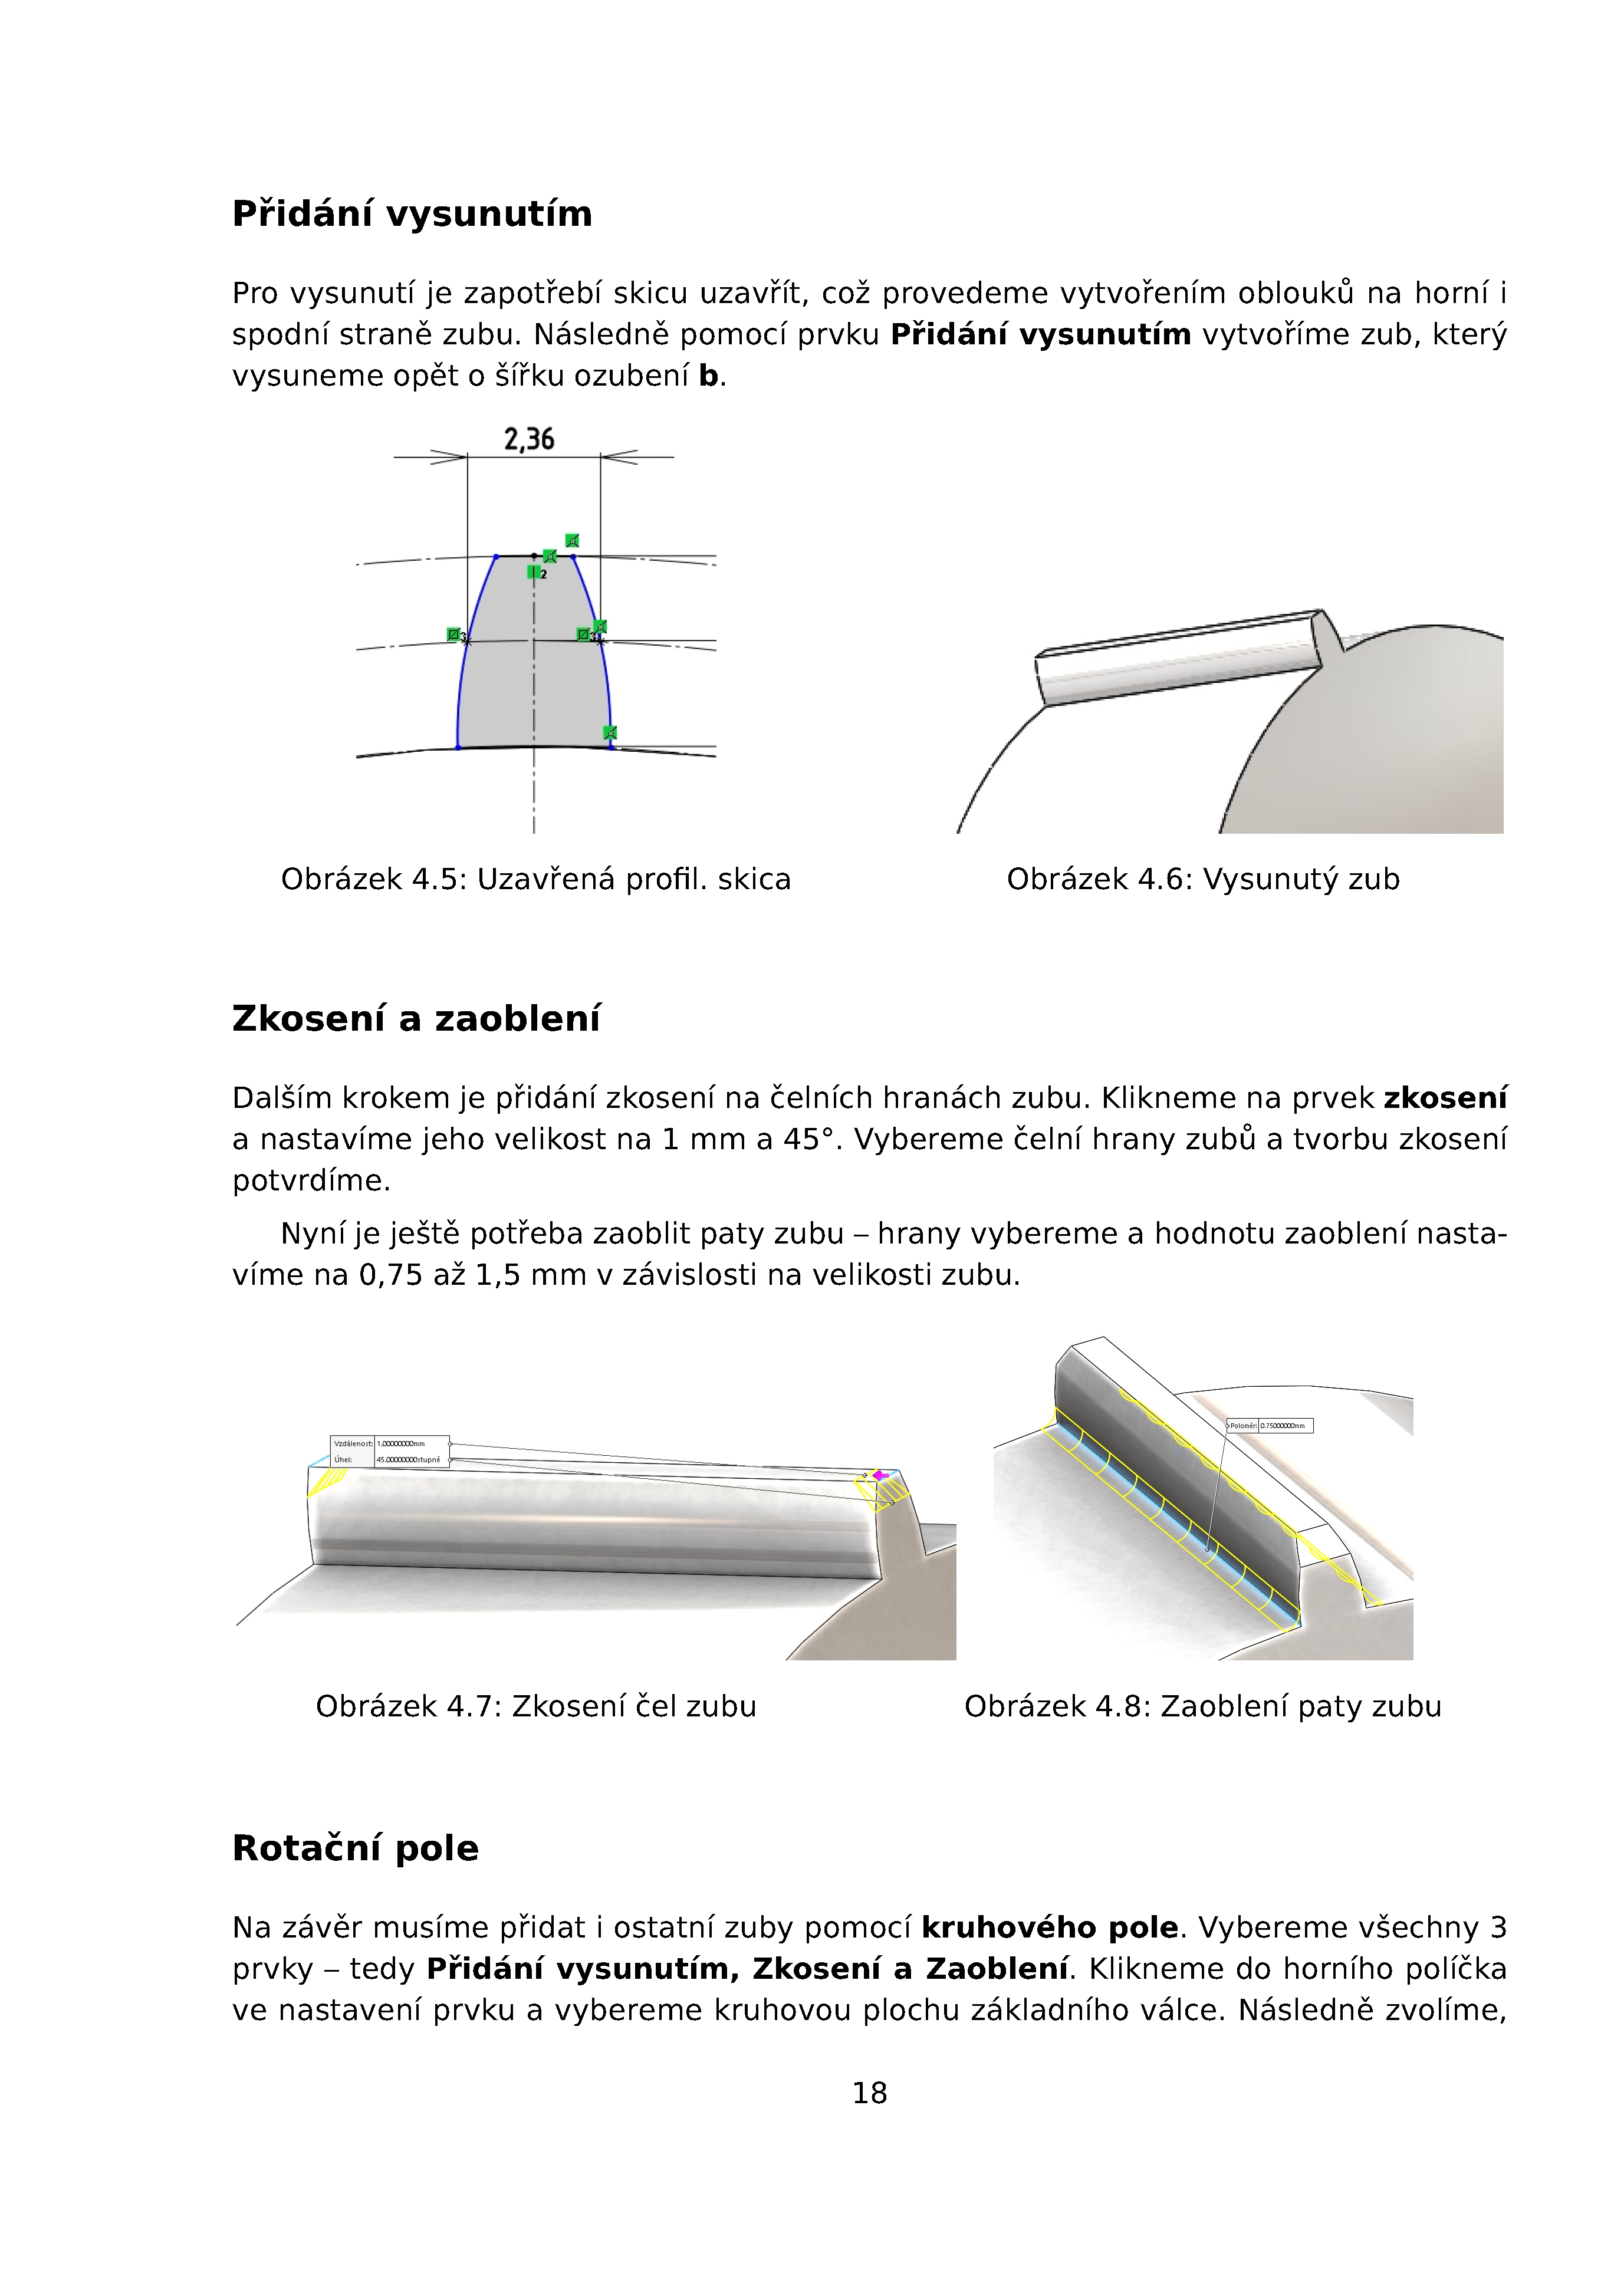
\includegraphics[width=0.7\textwidth]{img/020/guide1.png}
        \caption{Tištěné materiály}
        \label{fig:auxmat1}
    \end{minipage}
    \qquad
    \begin{minipage}[b]{0.45\textwidth}
        \centering
        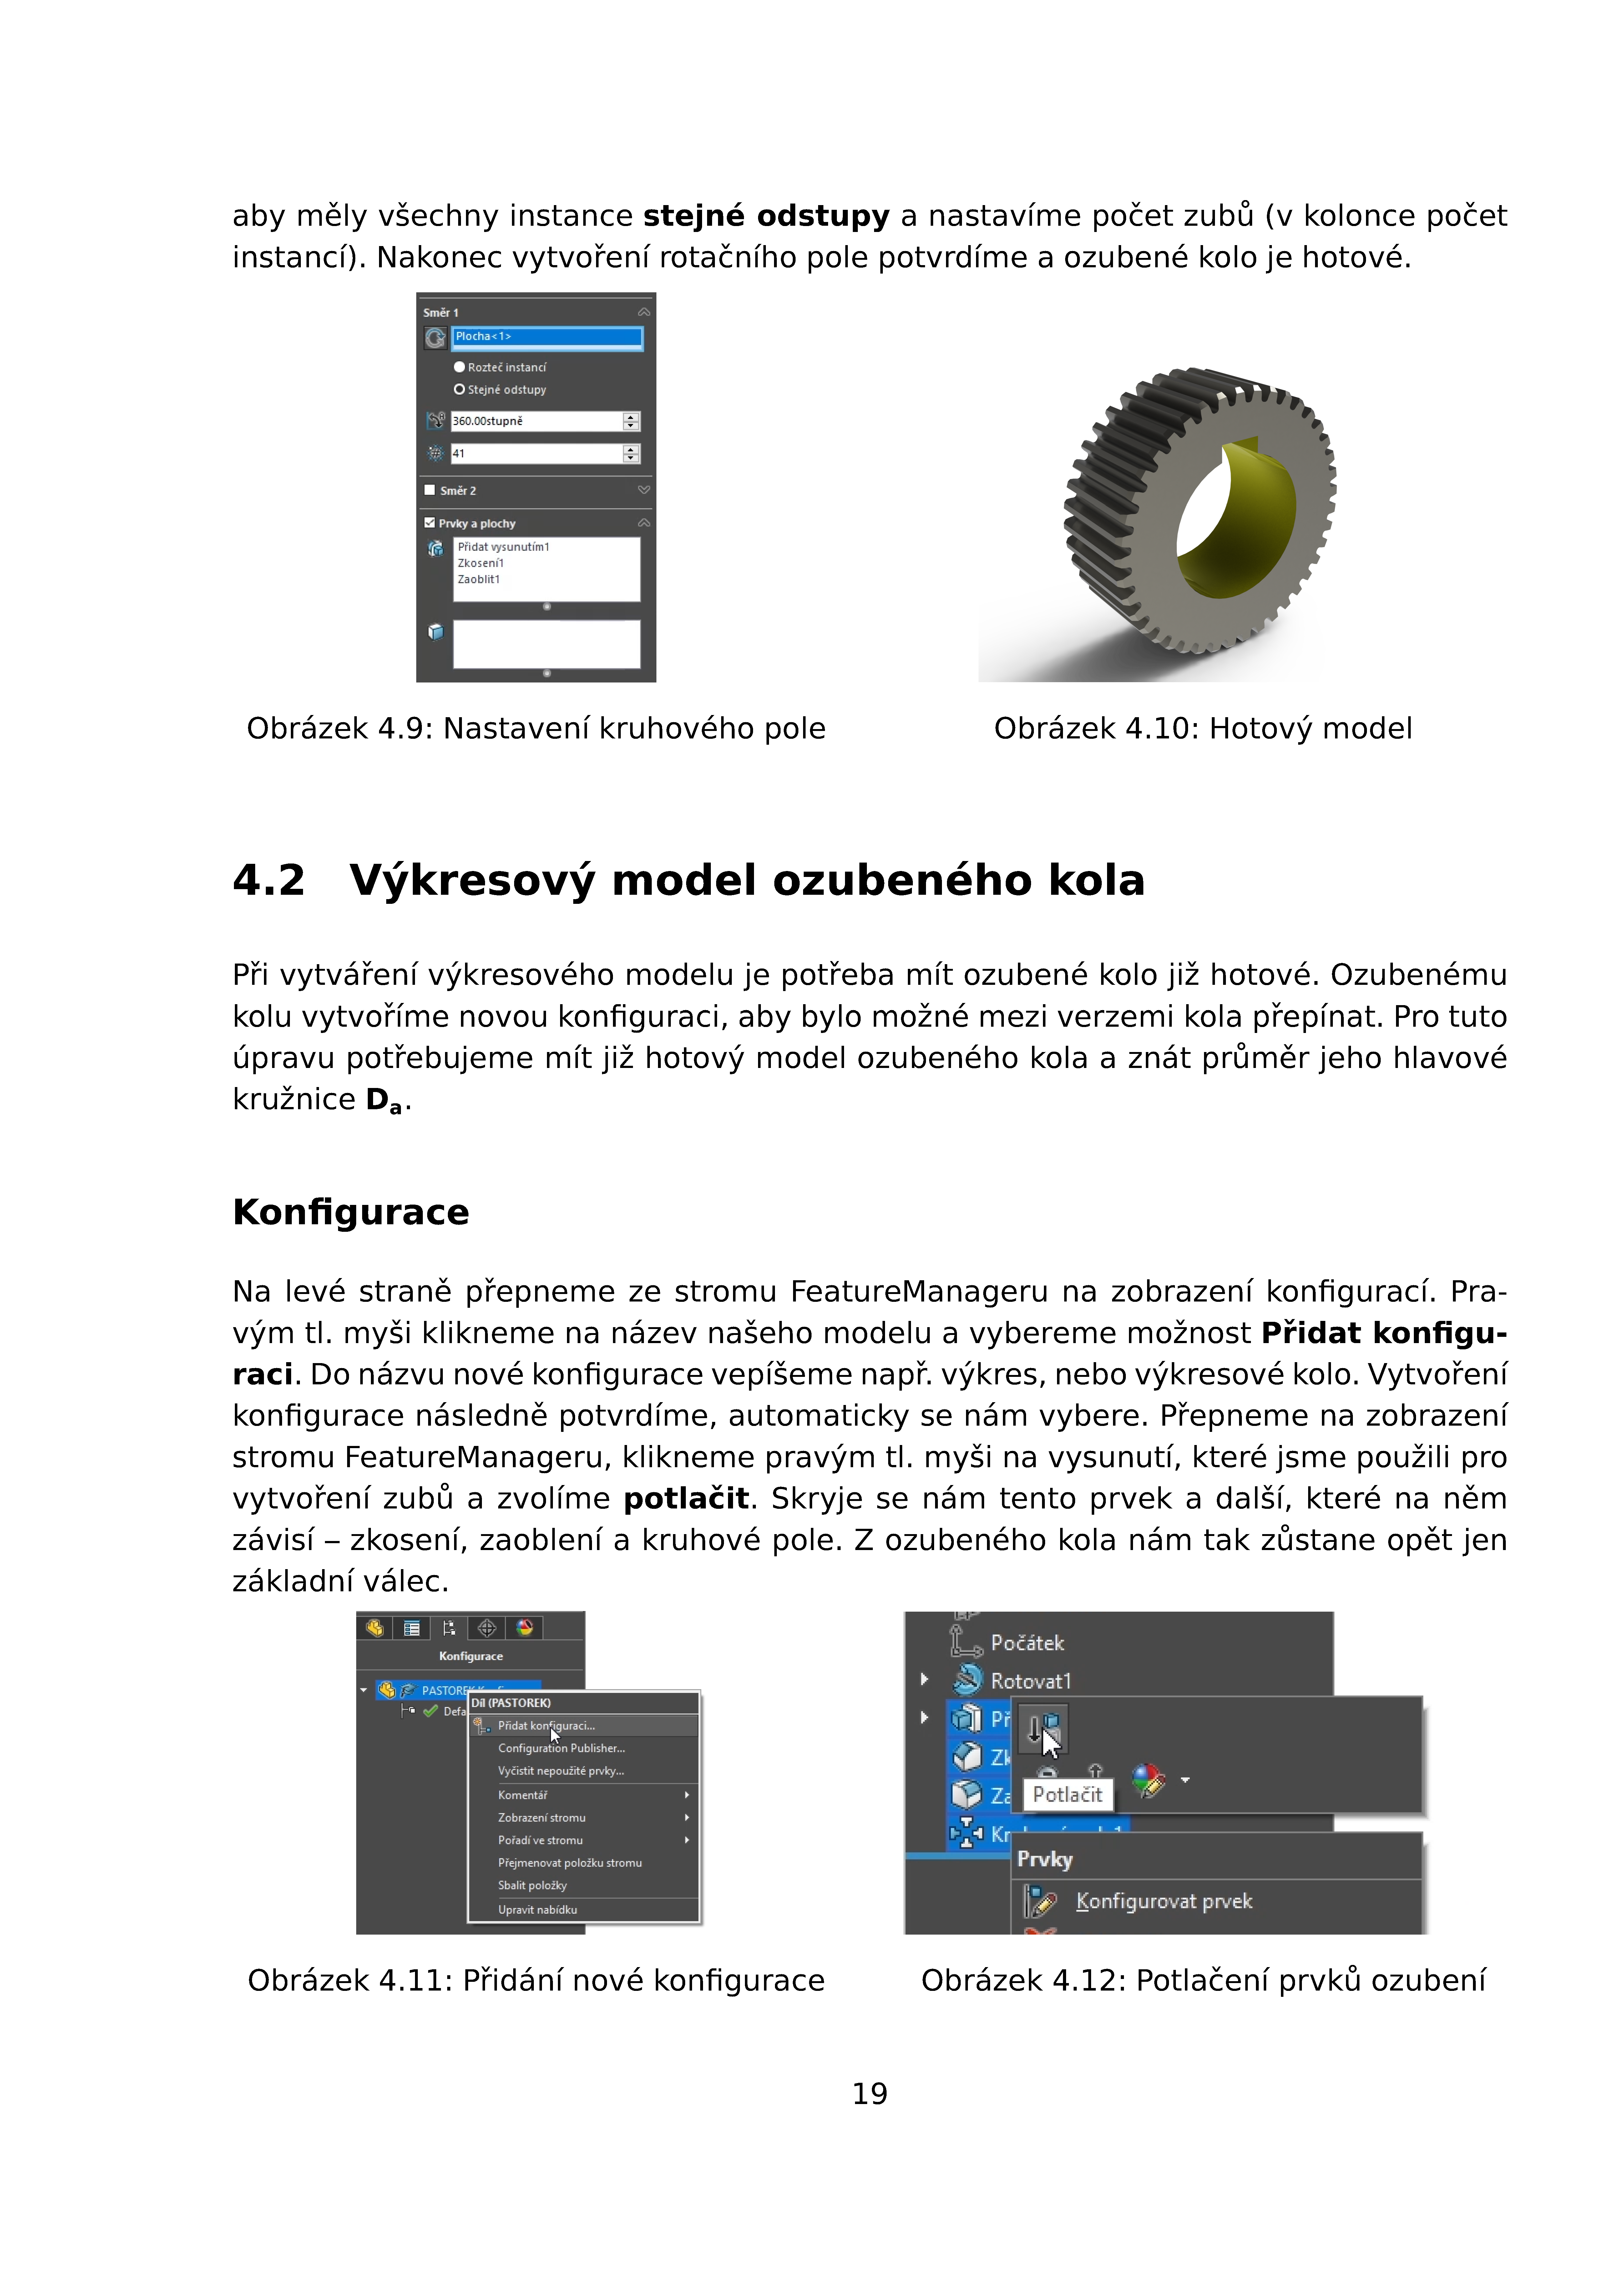
\includegraphics[width=0.7\textwidth]{img/020/guide2.png}
        \caption{Tištěné materiály}
        \label{fig:auxmat2}
    \end{minipage}
\end{figure}

\subsection{Struktura tisknutelných materiálů}
Z vlastní zkušenosti vím, že zorientovat se v dlouhých textech může být pro studenta poněkud obtížné.
Snažil jsem se pro to, aby byla orientace v tisknutelných materiálech co nejjednodušší.
Jednotlivé kategorie návodů jsou rozděleny do kapitol.
Každý návod je poté oddělen samostatným číslovaným nadpisem a rozdělen do několika menších, dílčích kroků.
Delší bloky textu jsem se pomocí ilustrací snažil rozdělit na menší odstavce.
Za zmínku stojí také tučné zvýraznění názvů prvků a používaných hodnot napomáhající přehlednosti.

\subsection{Otázky a úkoly}
Na konci každého návodu na 3D modelování jsou umístěny doplňující otázky a úkoly, které studentům umožňují si procvičit postupy, nebo ověřit získané znalosti.
U~většiny návodů z~ostatních kategorií není zapotřebí znalosti ověřovat, jelikož se jedná o~postupy, které studenti mohou používat, nicméně nejsou pro úspěšnou práci v~SolidWorks nutné.
Otázek a úkolů jsou záměrně umístěna v~sekci pro vyučující, která tvoří přílohu těchto tištěných materiálů.

\subsection*{Doporučení pro vyučující}
Součástí tisknutelných materiálů pro vyučující jsou i doporučení pro využívání materiálů a upozornění na potenciálně problematické části postupu.

\subsection{Dostupnost tisknutelných materiálů}
Verze tisknutelných materiálů bez řešení úloh je volně k~dispozici na webu \href{https://www.p3dportal.cz}{www.p3dportal.cz} v~sekci \enquote{Ke stažení}.
O~variantu pro vyučující je možné si zažádat na e-mailové adrese \href{mailto:info@pxmedia.cz}{info@pxmedia.cz}.

\section{Výukový portál P3D}
S~narůstajícím počtem videí a dalších doplňujících materiálů začal vznikat problém v~přehlednosti a uváděním jasných souvislostí.
Po delším přemýšlení jsem dospěl k~závěru, že nejjednodušší řešení bude vytvořit pro projekt vlastní webové stránky.
Díky nim si mohou nejen studenti, ale i vyučující najít celou výukovou sadu snadno a přehledně na jednom místě online.

Webové stránky jsem založil na redakčním systému WordPress, díky čemuž jej lze velmi snadno a rychle spravovat, nebo přidávat nový obsah.

\subsection{Design webu}
Stejně jako u~videí jsem se zaměřil na to, aby byl design webového portálu moderní a čistý.
Pozadí a většina prvků webu je laděné do tmavých barev.
Toto rozhodnutí jsem učinil z~několika důvodů.
Jednak je sledování menšího počtu světlejších elementů na tmavém pozadí příjemnější pro oči (zvláště v~pozdních hodinách) a jednak jsou v~dnešní době tmavé vzhledy u~aplikací a webových stránek velice populární.
Dále jsem vycházel z~mé vlastní preference tmavých barev.

Volba ostatních barev vychází z~designu náhledových obrázků videí, opět pro zachování konzistence.

\subsection{Struktura webu}
Pro přehlednost jsem stránky na webu rozdělil do tří úrovní. 
V~rámci celé struktury je pro snadnou navigaci zobrazena lišta s~odkazy pro snadný přesun mezi stránkami.

\noindent\B{Úvodní stránka} funguje jako rozcestník k~jednotlivým podstránkám. Je rozdělena na několik sekcí. V~horní části se nachází úvodní grafika. Níže jsou k~vidění dvě nejnovější videa vytvořená v~rámci celého projektu P3D. Ještě níže jsou poté viditelné všechny kategorie videí. (Viz obrázky \ref{fig:p3dportal-hp1}, \ref{fig:p3dportal-hp2} a \ref{fig:p3dportal-hp3})

\noindent\B{Kategorie} jsou na webu aktuálně čtyři -- 3D modelování, sestavy, výkresová dokumentace a instalace a nastavení. Na stránce každé kategorie jsou zobrazeny náhledové obrázky všech videí, které do dané kategorie patří. (Viz. \autoref{fig:p3dportal-cat})
Při kliknutí na některý z~náhledových obrázků se otevře detail daného videa. 

\noindent\B{V detailu videa} je zobrazený jeho popis, potřebné hodnoty a parametry (pokud nějaké jsou) a doplňkové úkoly a otázky vč. jejich řešení. Úkoly s~otázkami zobrazenými na detailu videa jsou jiné, než úkoly v~tisknutelných materiálech. Nehrozí tak, že by si student odpověď našel na webu. (Viz obrázky \ref{fig:p3dportal-3D} a \ref{fig:p3dportal-assembly})

\begin{figure}[htbp]
    \centering
    \begin{minipage}[b]{0.45\textwidth}
        \centering
        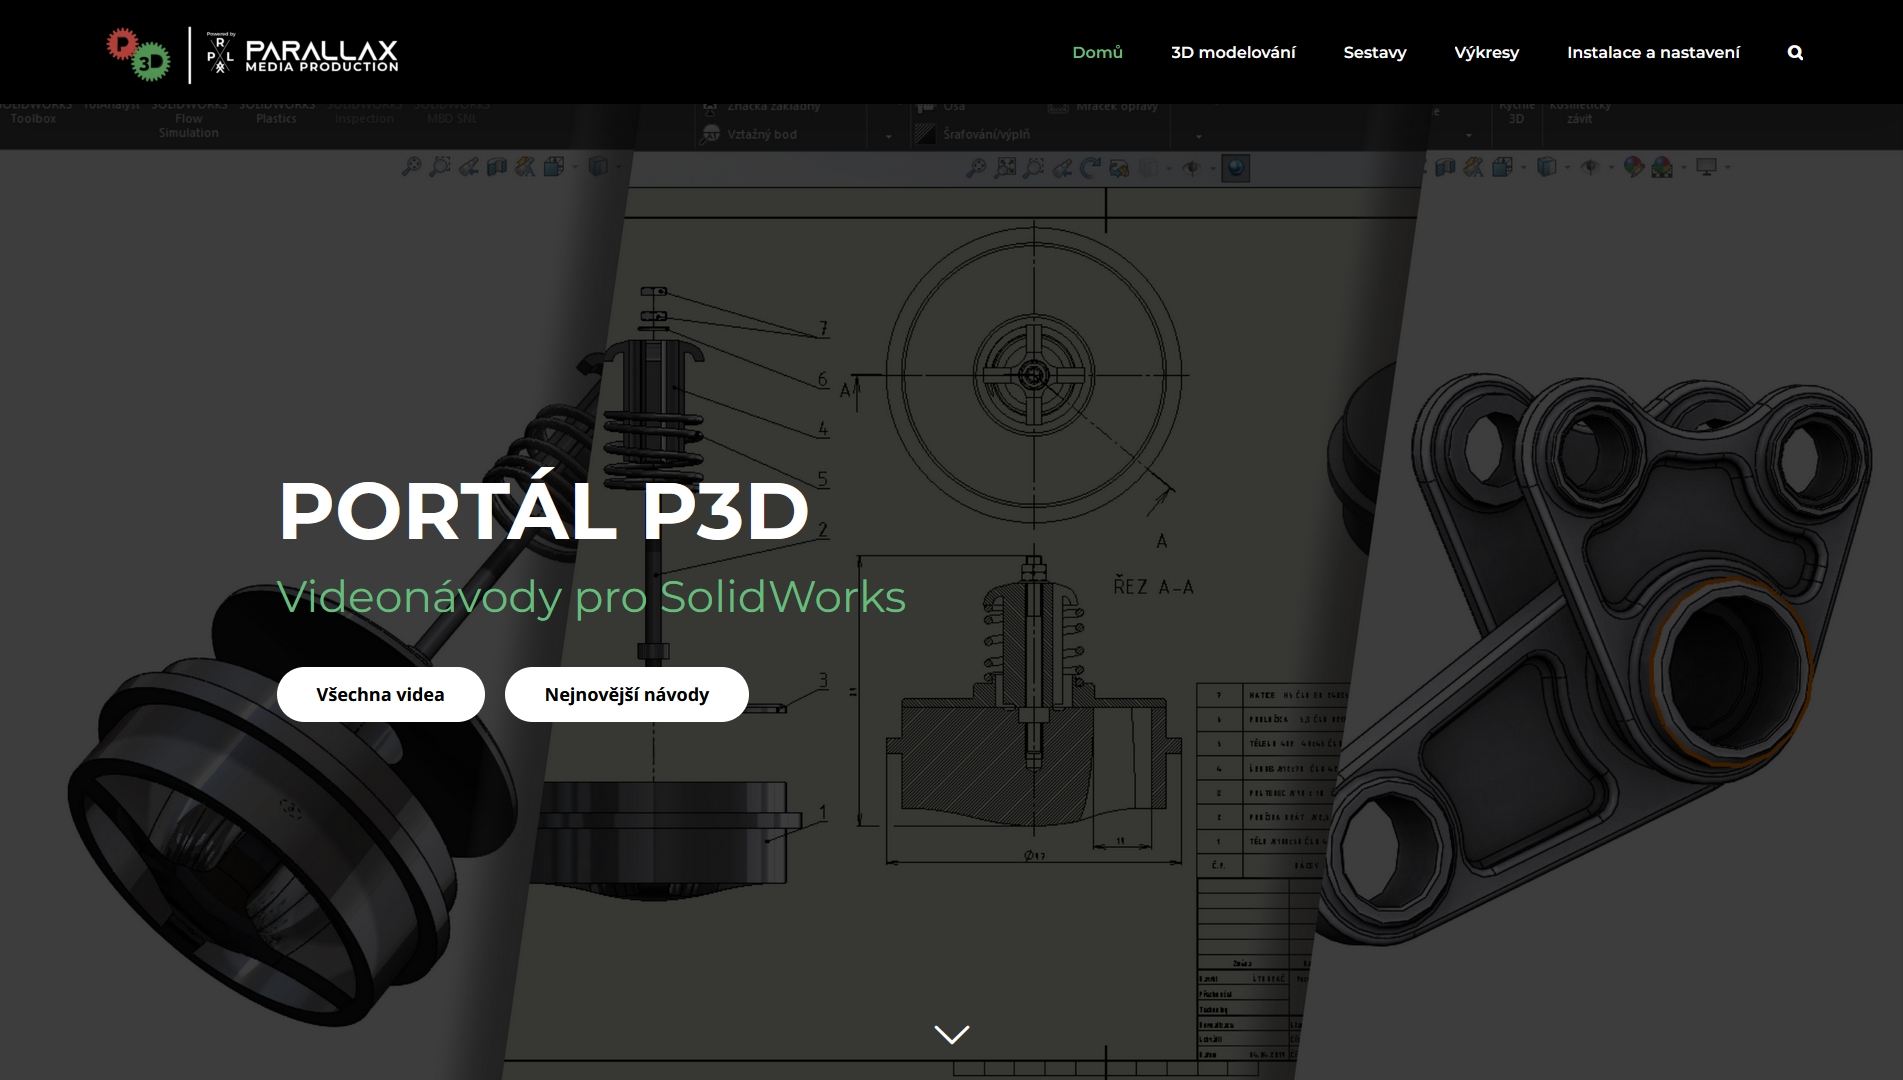
\includegraphics[width=1\textwidth]{img/020/web/web-hp1.png}
        \caption{Úvodní grafika webu}
        \label{fig:p3dportal-hp1}
    \end{minipage}
    \qquad
    \begin{minipage}[b]{0.45\textwidth}
        \centering
        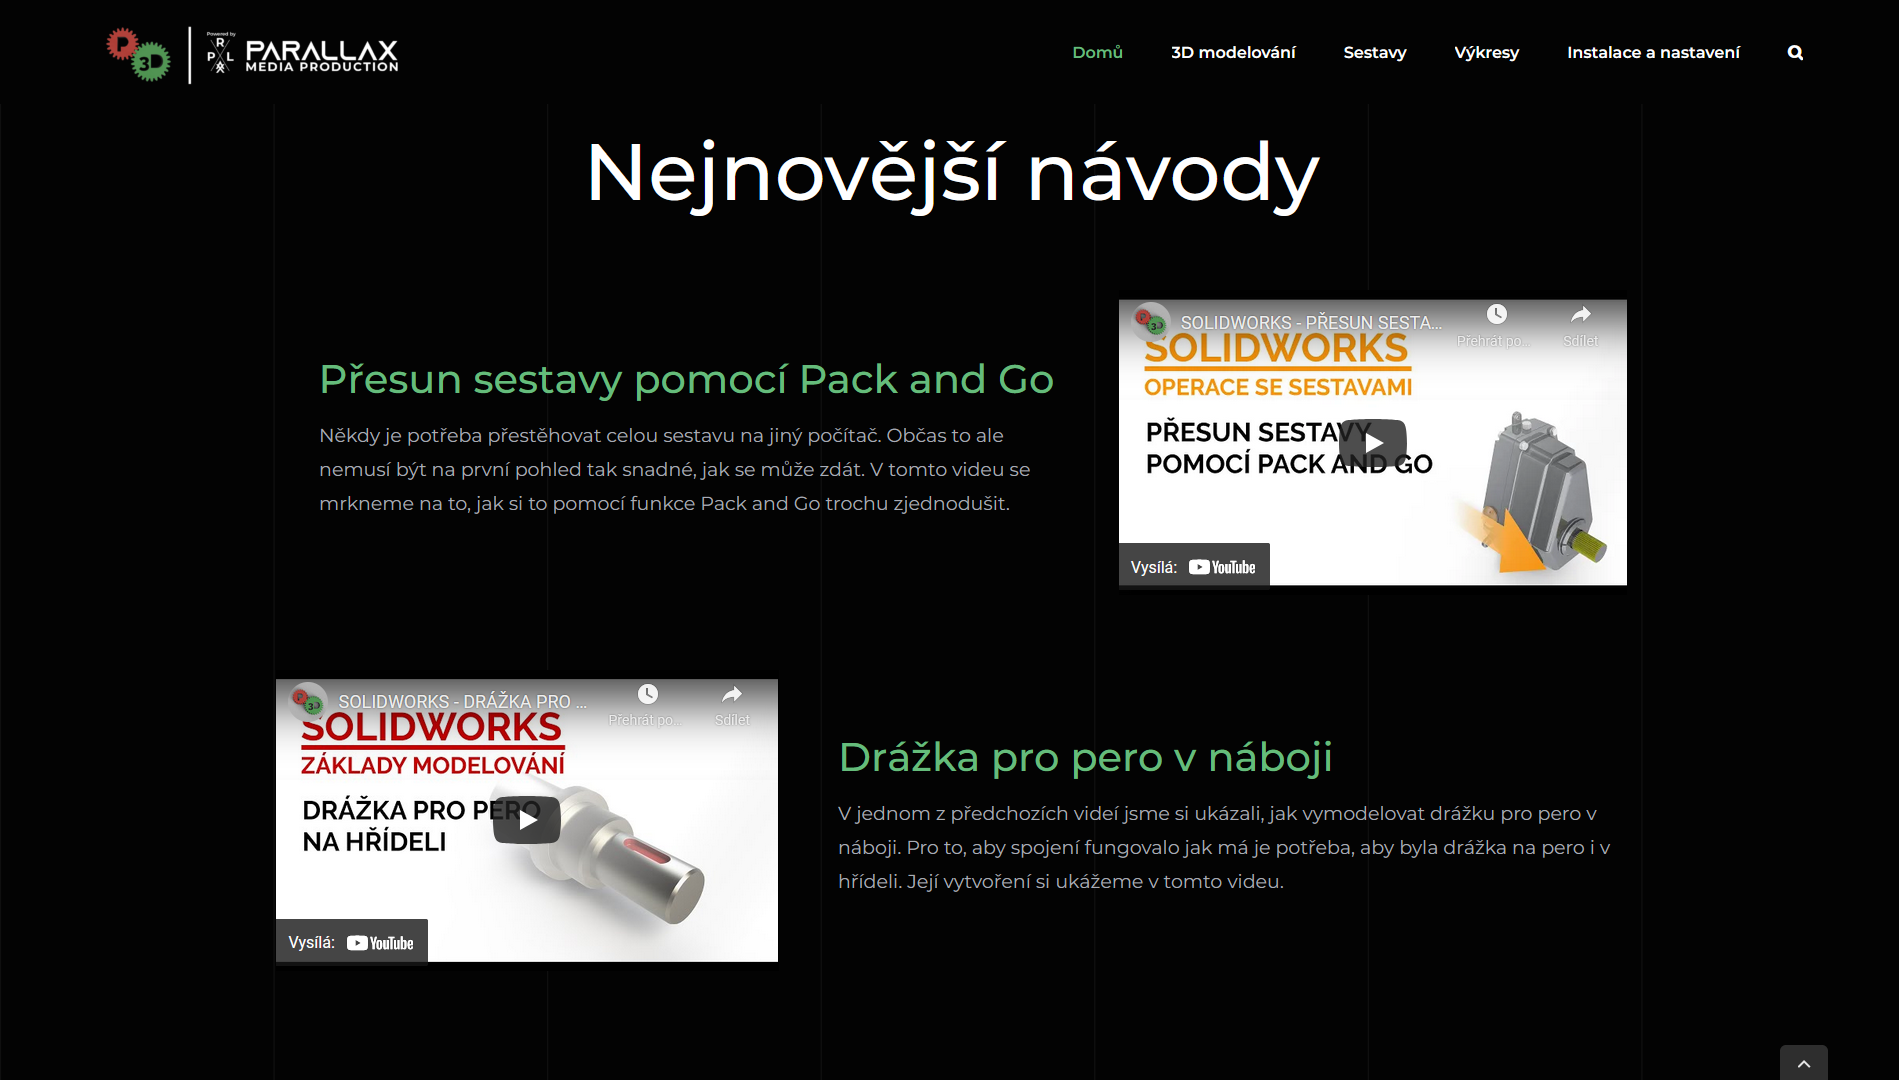
\includegraphics[width=1\textwidth]{img/020/web/web-hp2.png}
        \caption{Sekce \enquote{Nejnovější videa}}
        \label{fig:p3dportal-hp2}
    \end{minipage}
\end{figure}


\begin{figure}[htbp]
    \centering
    \begin{minipage}[b]{0.45\textwidth}
        \centering
        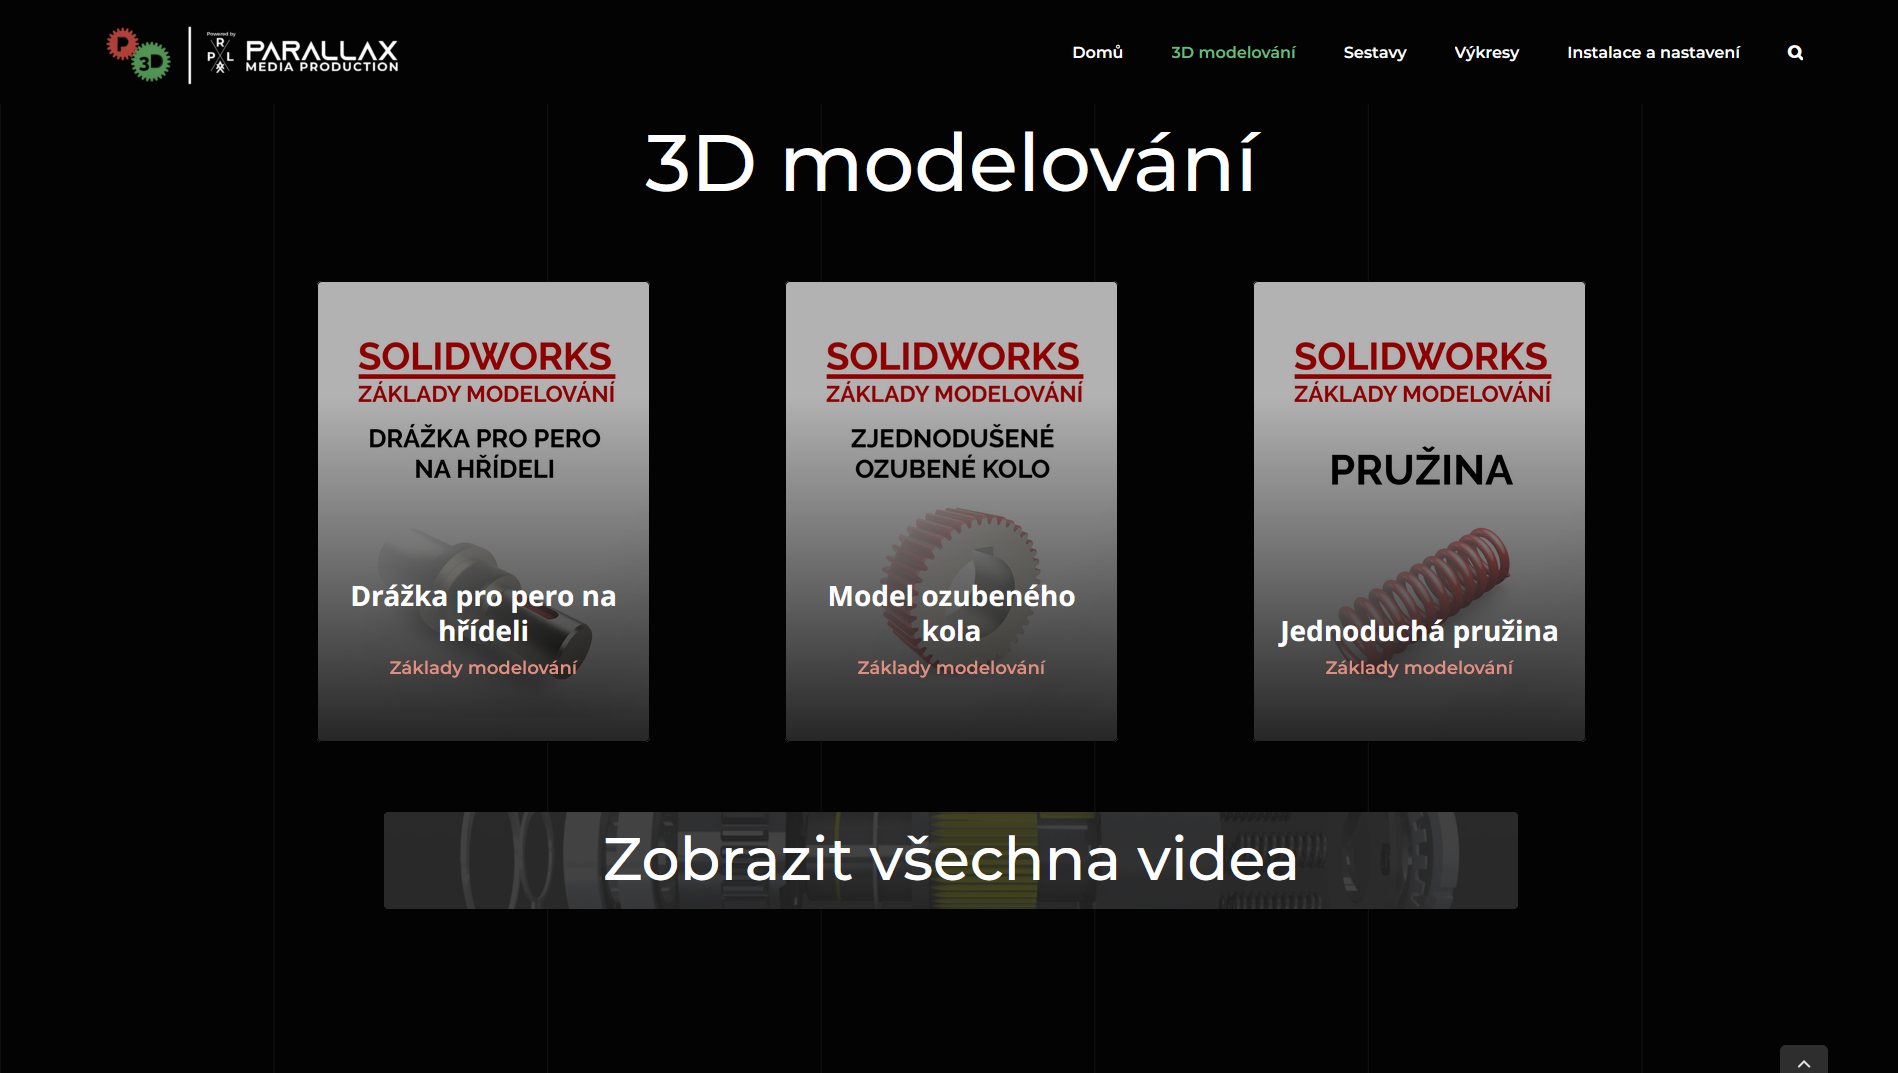
\includegraphics[width=1\textwidth]{img/020/web/web-hp3.png}
        \caption{Úvodní grafika webu}
        \label{fig:p3dportal-hp3}
    \end{minipage}
    \qquad
    \begin{minipage}[b]{0.45\textwidth}
        \centering
        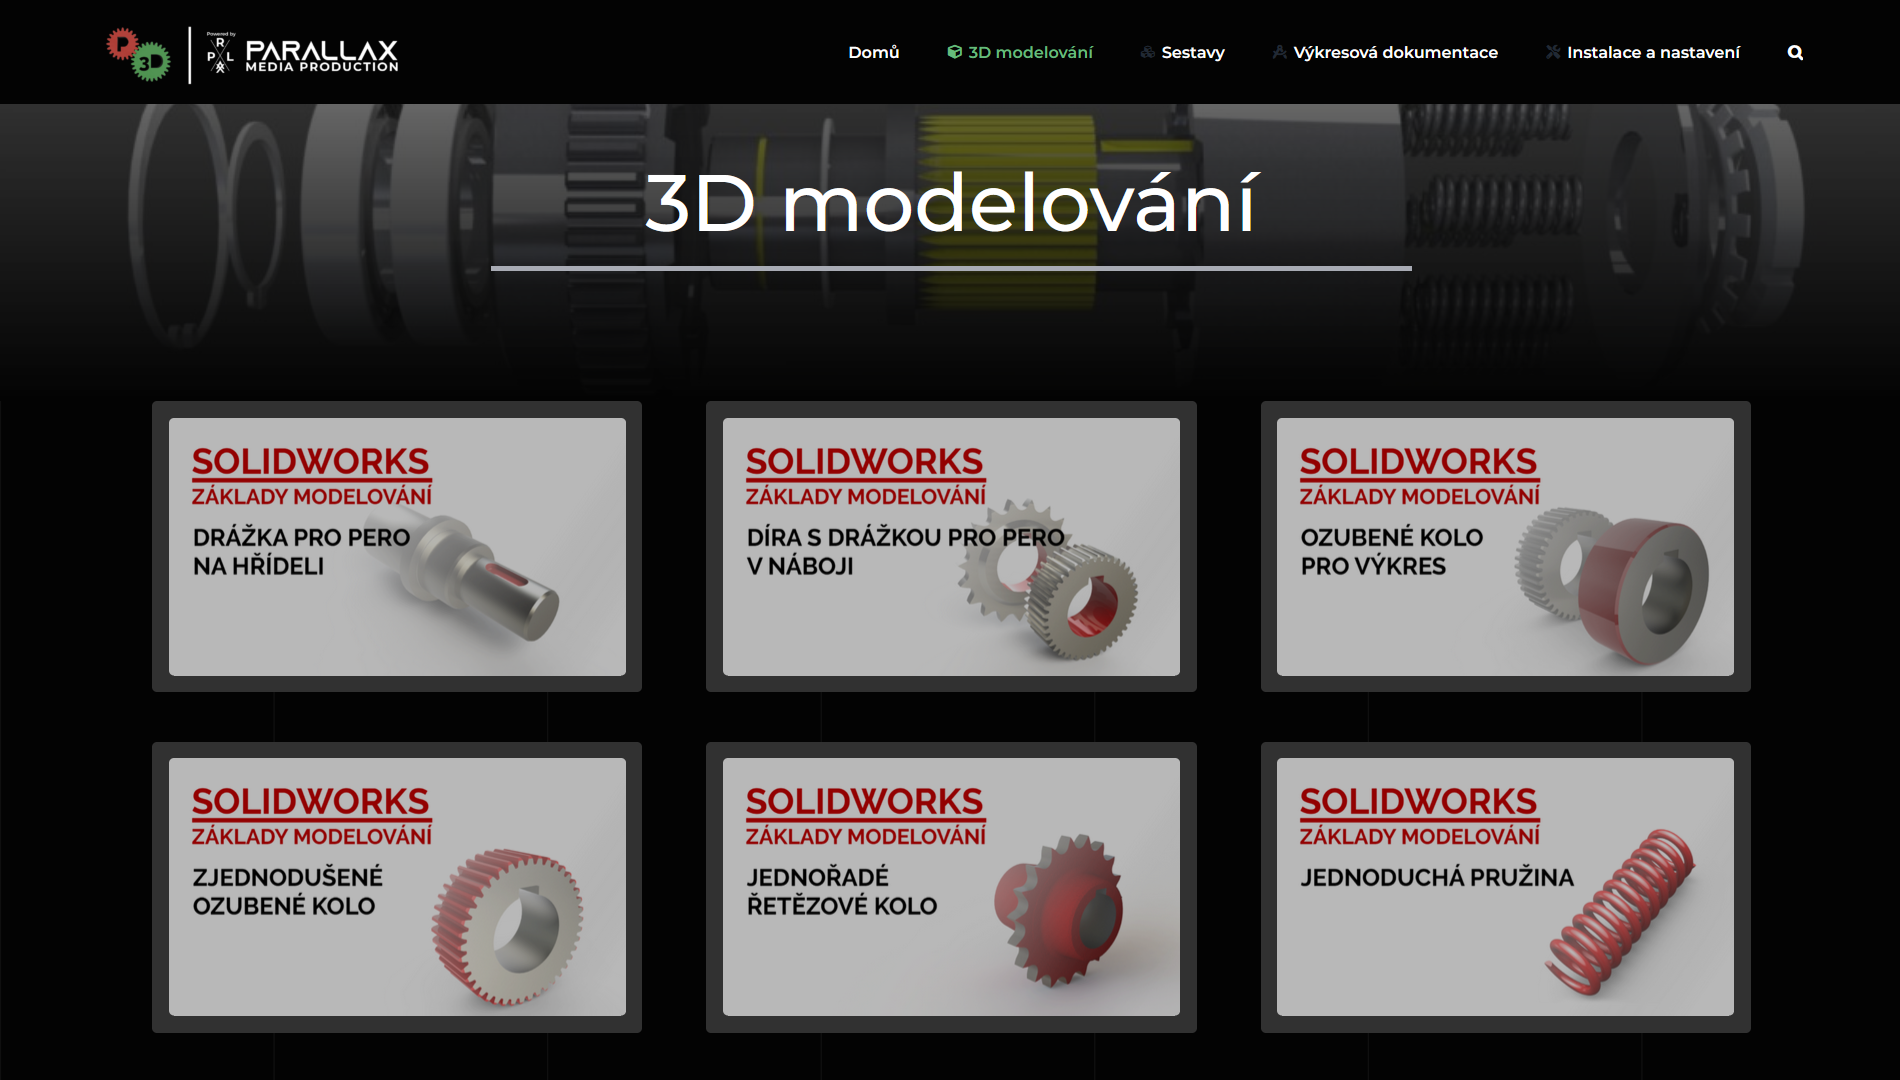
\includegraphics[width=1\textwidth]{img/020/web/web-cat.png}
        \caption{Zobrazení celé kategorie}
        \label{fig:p3dportal-cat}
    \end{minipage}
\end{figure}

\begin{figure}[htbp]
    \centering
    \begin{minipage}[b]{0.45\textwidth}
        \centering
        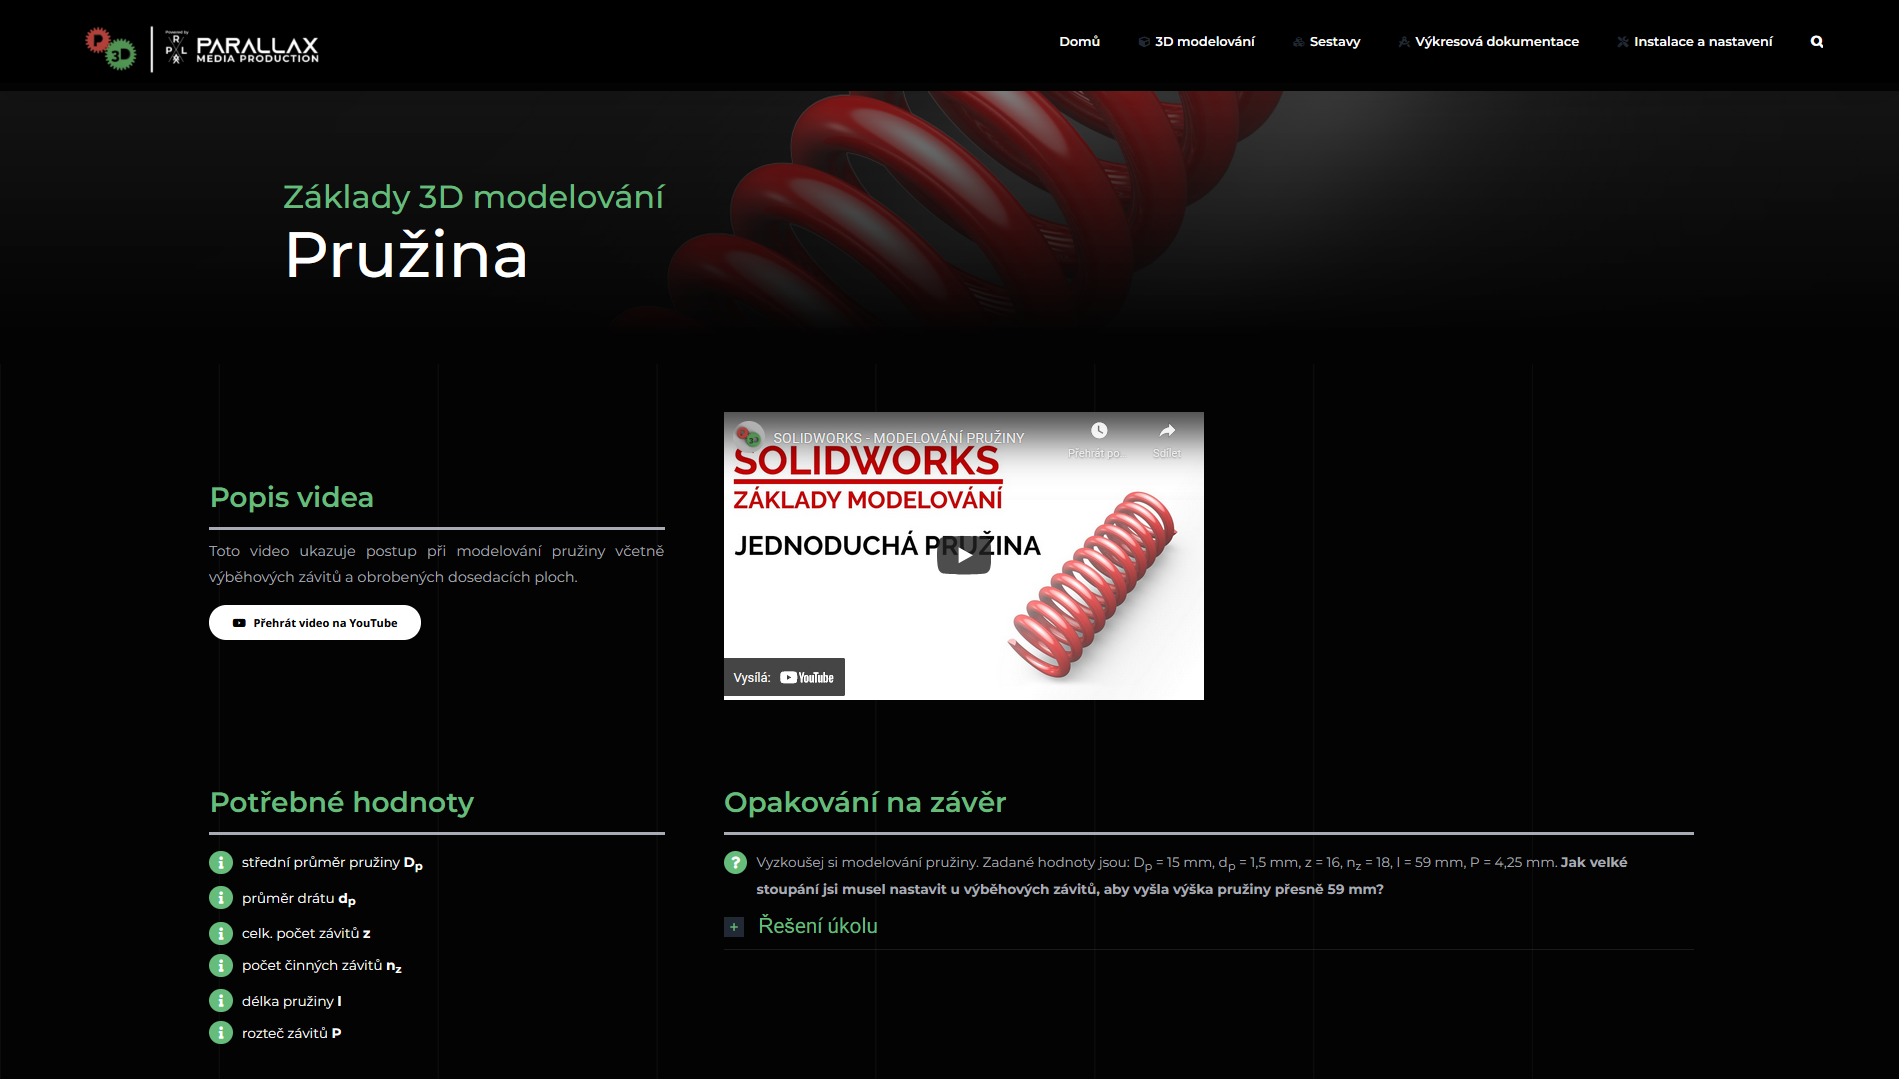
\includegraphics[width=1\textwidth]{img/020/web/web-3D.png}
        \caption{Detail videa}
        \label{fig:p3dportal-3D}
    \end{minipage}
    \qquad
    \begin{minipage}[b]{0.45\textwidth}
        \centering
        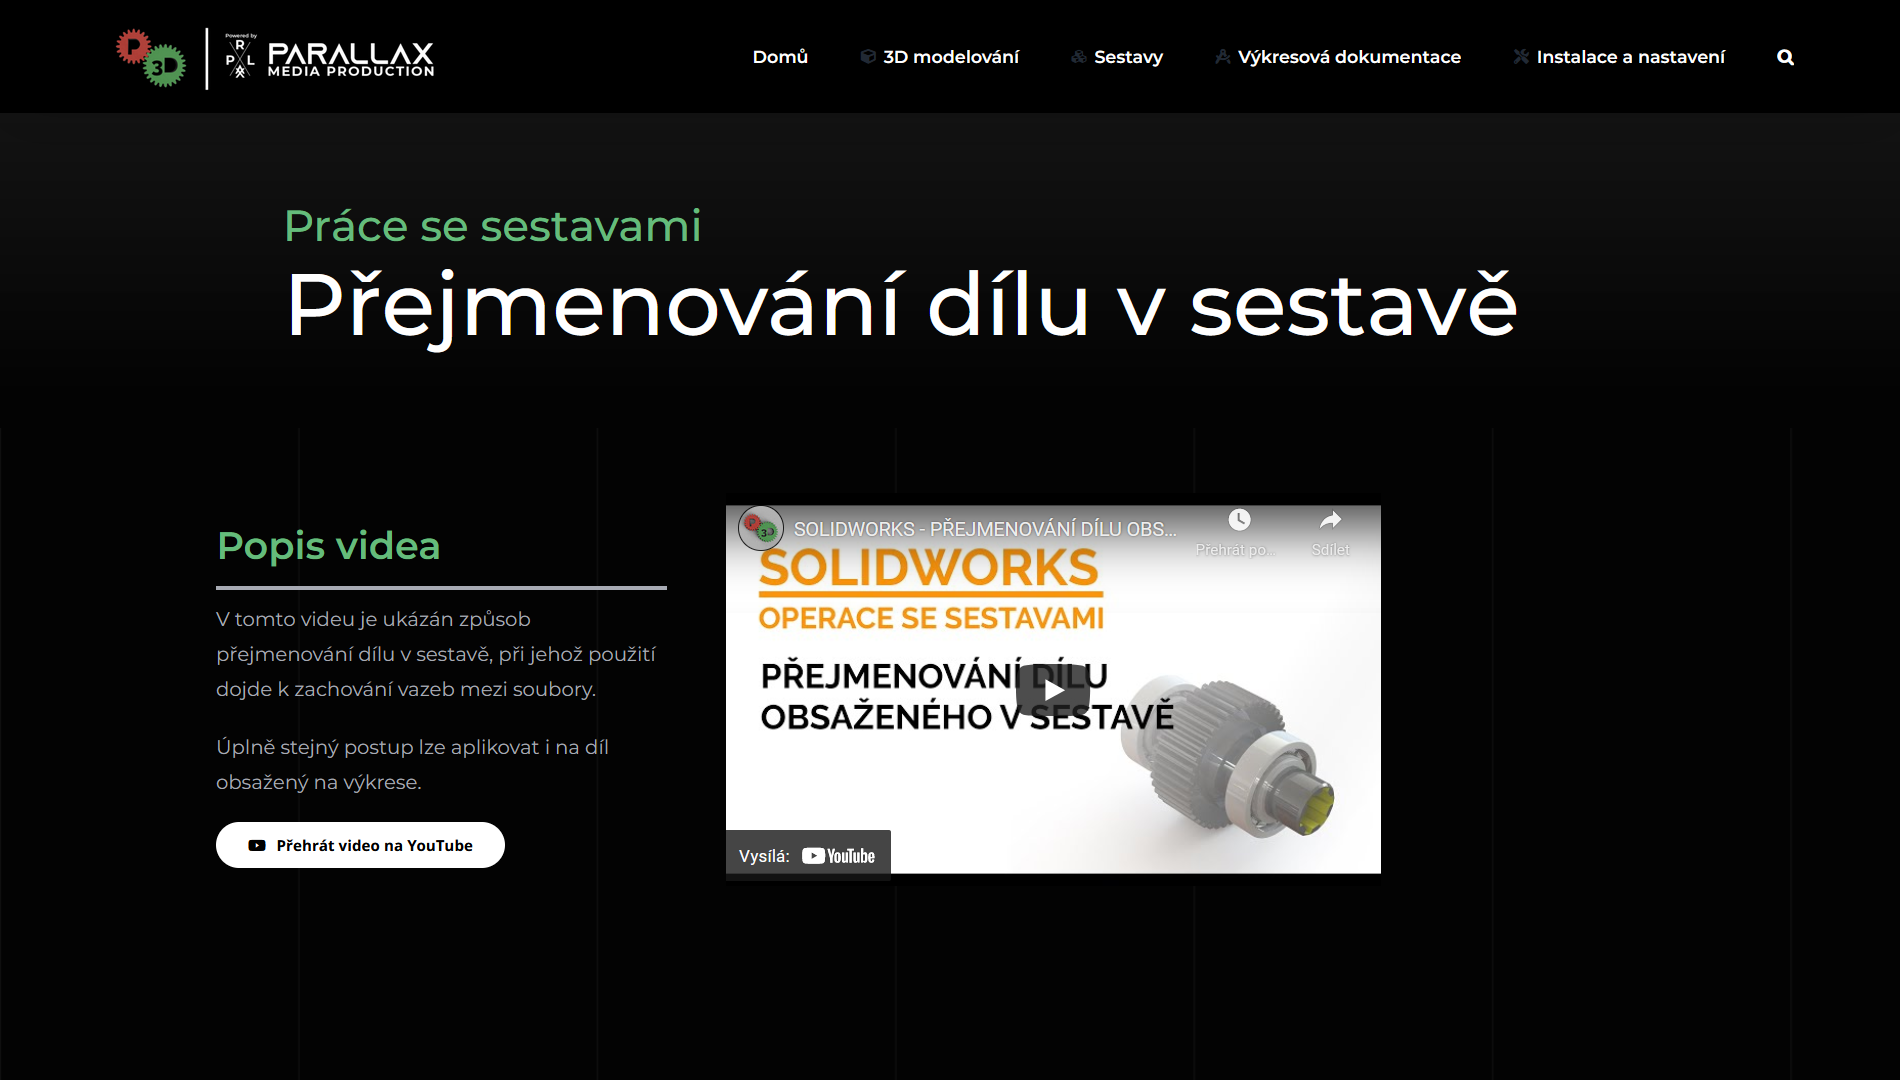
\includegraphics[width=1\textwidth]{img/020/web/web-assembly.png}
        \caption{Detail videa}
        \label{fig:p3dportal-assembly}
    \end{minipage}
\end{figure}

\subsection{Zkracovací subdoména go.p3dportal.cz}
Přestože jsou všechny odkazy na webu snadno čitelné\footnote{Sestávají se z~dobře čitelných částí slov, nikoliv náhodných řetězců znaků}, kvůli struktuře webu mohou být příliš dlouhé.
Z~toho důvodu jsem vytvořil tzv. zkracovací subdoménu \href{https://go.p3dportal.cz}{go.p3dportal.cz}, která umožňuje jakémukoliv odkazu přiřadit jeho zkrácený alias.
Běh této funkce je zajišťován white-labelovým\footnote{Produkt, který si jeho uživatel může skrýt pod vlastní frontend, v~tomto případě doménu} zkracovačem \href{https://short.io}{short.io}.
Doména go.p3dportal.cz tak slouží čistě jako front end\footnote{Front end = vnější vrstva určité aplikace (to, co vidí uživatel), opakem je back end}.
